% 请在下方的大括号相应位置填写正确的节标题和标签,以及作者姓名
\section{*数组}\label{sec:数组}
\sectionAuthor{Jiaqi Z.}

% 请在下方的item内填写本节知识点
\begin{Abstract}
    \item 如何初始化定义数组
    \item 如何调用数组的元素
    \item 如何定义“关联数组”
\end{Abstract}

在上一节的最后,我们提到:需要有一种手段保存所有的元素。这在当时是一种可选的手段,除此之外,还有一个更常见的例子:假设我们现在需要计算一个班级所有同学考试的平均分,并在最后输出高于平均分的分数。此时,寻找一个方法用来存放所有数据就是必要的了。而与其他编程语言类似,在bash脚本中,也有类似于“数组”这样的数据结构。

在本节,我们将介绍如何在程序中显式定义\footnote{这里所说的“显式定义”,指的是在程序代码中直接写明数组变量的值}一个数组,以及如何调用数组的元素;在最后,我们再简单讨论一下\emph{关联数组}的内容,这是一个类似于Python中“字典”的哈希表(Hash Map)结构。

\subsection{定义数组}\label{subsec:数组-定义数组}

定义数组的方法并不困难,其基本格式为\code{<变量名>=(value1 value2 value3 ...)},其中数组变量元素整体用小括号括起来,且各个元素之间用空格间隔。例如,下面的程序我们定义了一个数组:

\begin{lstlisting}[language=bash,numbers=left,caption={array\_test}]
#!/bin/bash
# 定义数组
array1=(1 2 3 4 5)
array2=("Hello" "World")
array3=("Hello" 3 true)
\end{lstlisting}

在这段代码中,我们定义了三个数组,第一个数组\code{array1}和第二个数组\code{array2}分别是由数字和字符串组成的数组。在bash脚本中,数组不仅仅可以是数字,也可以是字符串或者其他数据类型。与C语言固定数组类型不同,在bash脚本中,一个数组内可以有多个数据类型,正如\code{array3}数组所演示的那样,其中可以包括字符串、数字、甚至逻辑值,都是可以放在一个数组变量下。

\begin{attention}
    在定义数组时,与C语言不同,bash脚本不需要提供数组长度。换句话说,bash脚本的数组是\emph{可变长度}的数组。

    而且,与其他编程语言不同,bash脚本仅支持\emph{一维数组}。
\end{attention}

\subsection{数组调用}\label{subsec:数组-数组调用}

与C语言类似的是,数组调用也是采用\code{<数组名>[下标]}的格式,其中下标是使用\emph{中括号}括起来。一般数组的调用分为“读取”和“写入”两种情况,我们将依次讨论这两种情况的区别。

\begin{attention}
    一个很关键的事情是:数组下标始终是\emph{从0开始计数}的,即\code{array1[0]}表示数组\code{array1}的第一个元素。这件事情几乎是当今所有编程语言的基础\footnote{这一切是从C语言开始的。}
\end{attention}

\subsubsection{读取调用}

下面的代码演示了如何读取数组的元素:

\begin{lstlisting}[language=bash,numbers=left,caption={array\_test\_cont1}]
#!/bin/bash
# 定义与调用数组
array1=(1 2 3 4 5)
array2=("Hello" "World")
array3=("Hello" 3 true)
# 调用数组
result=$(( ${array1[0]}+${array1[1]} )) 
echo $result
echo ${array2[0]}
if [ ${array3[2]} ]; then
    echo ${array3[0]}
fi
\end{lstlisting}

上面代码的第7、9、10行分别演示了三种常见的调用方式,分别是\emph{在表达式中调用;在语句中调用;在逻辑表达式中调用}。可以发现,无论哪一种调用方式,其格式基本是一样的,因此,读者完全不必将其分类到如此精确的程度,只需要记住一个原则:\emph{在读取时需要加\$符号和大括号}即可。

\subsubsection{写入调用}

在必要的时候,我们也可以对已有的数组进行修改。例如,下面的代码是对上面代码的进一步补充,并在其中演示了如何修改数组的元素值:

\begin{lstlisting}[language=bash,numbers=left,caption={array\_test\_cont2}]
#!/bin/bash
# 定义与调用数组
array1=(1 2 3 4 5)
array2=("Hello" "World")
array3=("Hello" 3 true)
# 调用数组
array1[0]=5
result=$(( ${array1[0]}+${array1[1]} )) 
array1[5]=$result
result[1]=${array2[0]}
if [ ${array3[2]} ]; then
    array3[2]=false
fi
result[2]=${array3[2]}
for i in {0..2}
do
    echo ${result[$i]}
done
\end{lstlisting}

在程序的第8行,我们将数组元素当作一般的变量,并对其进行赋值。但稍有难度的是第9行和第10行,其中第9行明明数组的最大下标为4(想想为什么5个元素的最大下标为4),但我们却可以对下标为5的元素赋值。在bash脚本中,这可以视作\emph{添加元素}。与Python等语言可能还需要类似于\code{append()}函数不同,bash脚本只需要如同正常的数组进行操作即可,程序会自动追加新的元素在对应的位置。

更奇怪的是第10行代码:为什么\code{result}明明是一个普通变量,却可以带有下标追加新的元素?事实上,一个普通的变量也可以看作是一个\emph{长度为1的数组}。正因如此,我们可以对普通变量如同数组般进行操作(追加新的元素),甚至对于普通的变量,例如定义了变量\code{a=5},我们也可以使用\code{a[0]}来代表这个变量。

\begin{extend}
    我们可以将整个数组看作一个一维的表格,其编号从0开始,每创建一个元素,就在对应位置加上内容。因此,你可以将下标设置成不连续的(例如,\code{array1[10]}是允许的,此时的数组如图\ref{fig:数组-添加数组元素后数组内元素的值}所示)

    \begin{figure}
        \centering
        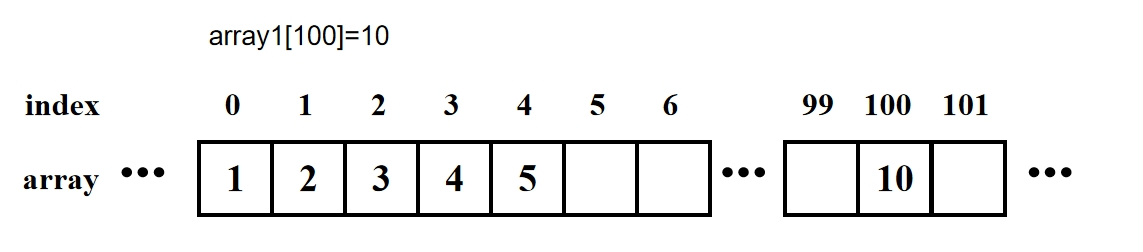
\includegraphics[width=1\linewidth]{Linux基础/Shell脚本基础/数组/fig/数组结构.png}
        \caption{添加数组元素后数组内元素的值}
        \label{fig:数组-添加数组元素后数组内元素的值}
    \end{figure}

    正如图中所示的那样,数组前面也可以有元素(负下标),但这些除非特殊情况,否则不建议使用。同样,也正如你所见,对于没有的元素,其变量值为“空”。
\end{extend}

除此之外,还有一些特别的方法对数组进行调用。例如,借助于\code{*}符号,我们可以获取数组内所有元素的值(其方法为\code{<变量名>[*]};使用\code{\#}符号可以获取数组的长度。例如,对于数组\code{array1},可以通过\code{\$\{\#array1[*]\}}的方式获取其数组长度。

\begin{extend}
    关于获取数组长度的方法,实际上近似等价于在介绍参数时(\ref{subsec:输入-参数输入})所提到的\emph{判断参数个数}的方法。也如同当时所介绍的方法一样,这里的\code{*}也可以换成\code{\@}符号。
\end{extend}

\subsection{*关联数组}\label{subsec:数组-关联数组}

\begin{extend}
    在创建数组时,默认都是以数字作为下标。类似于Python中的“字典”结构,在bash脚本中我们也可以创建带有“键值对”的哈希表结构,称为\emph{关联数组}。在定义关联数组前,需要使用\code{declare -A}的方式声明这个数组是关联数组。之后,就可以在下标中使用其他类型的数据(如字符串)对数组内的元素进行赋值。例如,下面的代码演示了如何定义与调用关联数组:

    \begin{lstlisting}[language=bash,numbers=left,caption={assosiative\_array}]
#!/bin/bash
# 定义与调用关联数组
declare -A data=(["name"]="Jiaqi Z.")
data["band"]="Roselia"
# 调用关联数组
echo "My name is ${data["name"]}, and I love ${data["band"]}."
    \end{lstlisting}

    在第3行,我们使用\code{declare -A}定义了一个“关联数组”,并在其中初始化了一个下标\footnote{在哈希结构中,我们通常称这个下标为“键”(key),而称这个数组的元素值为“值”(value)。}为“name”的元素,其值为“Jiaqi Z.”。

    在第4行,我们又如同调用一般的数组一样,对其进行赋值(追加了一个新的键)。之后在第6行调用了这个数组,并如同一般调用下标那样调用这个数组的“键”从而获得对应的“值”。

    需要注意的是:在初始化定义时,需要特别指明元素的键(其基本格式如上面代码第3行那样),而在后续的使用中,则完全可将其视为特殊的数组使用(调用)

    与前面所介绍的获取数组所有元素类似,对于“关联数组”而言,我们也可以使用\code{<变量名>[*]}的方式获得其所有元素的值。只不过在这里仅输出所有“值”(不包括“键”)。如果希望输出所有“键”的元素,可以在前面加感叹号(如\code{!<变量名>[*]})。例如,对于上面的代码,可以使用\code{echo \$\{data[*]\}}的方式输出所有值,使用\code{echo \$\{!data[*]\}}的方式输出所有“键”。
\end{extend}


% \subsection{错误处理}\label{subsec:节标题-错误处理}
% % 请在本节列出可能遇见的错误与解决方法

% \subsubsection{错误1}

% \subsubsection{错误2}

% \subsubsection{错误3}